
\subsection*{Phần 1: Sự rơi của một tảng đá}
\noindent Khoảng cách giữa bề mặt vật thể so với bề mặt Trái Đất và kích thước vật thể rất nhỏ so với bán kính Trái Đất, do đó, ta có thể coi lực hấp dẫn tác dụng lên vật thể có độ lớn không đổi và bằng $F=mg$. Một lực có độ lớn tương tự cũng sẽ tác dụng lên Trái Đất. \\

\noindent\textbf{1a.} Trong trường hợp này, khối lượng của vật rất nhỏ so với khối lượng Trái Đất nên ta có thể coi Trái Đất đứng yên trong suốt quá trình khảo sát. Thời gian rơi của vật được xác định bởi:
\begin{equation*}
  \tau_{a}=\sqrt{\frac{2h}{g}}\approx 4,5 \SI{ }{\second}
\end{equation*}

\noindent\textbf{1b.} Trong trường hợp này, khối lượng của vật và Trái Đất bằng nhau nên tâm của chúng chuyển động với vận tốc và gia tốc bằng nhau. Vật sẽ chạm đất sau khi nó diđược một đoạn $h/2$. Thời gian chuyển động là:
\begin{equation*}
  \tau_{b}=\sqrt{\frac{h}{g}}\approx 3,2 \SI{}{\second}
\end{equation*}

\noindent\textbf{2a.} Theo định luật bảo toàn năng lượng:
\begin{equation*}
  \frac{1}{2}mV^{2}=mgh\implies V=\sqrt{2gh}\approx \SI{45}{\metre\second^{-1}}
\end{equation*}

\noindent\textbf{2b.} Gọi $V_{1}$ là vận tốc mỗi vật tại thời điểm trước ta chạm, ta có:
\begin{equation*}
  \frac{h}{2}=\frac{V_{1}^{2}}{2g}\implies V_{1}=\sqrt{gh}
\end{equation*}
vận tốc của vật so với Trái Đất:
\begin{equation*}
  V=2V_{1}=2\sqrt{gh}\approx\SI{63}{\metre\second^{-1}}
\end{equation*}

\subsection*{Phần 2: Tàu vũ trụ}
\noindent\textbf{1.} Trong trường hợp khối lượng của tàu rất nhỏ so với khối lượng Trái Đất, ta có thể coi Trái Đất không di chuyển. Khi đó, tàu chuyển động theo quỹ đạo tròn có tâm trùng với tâm Trái Đất. Phương trình chuyển động của tàu là:
\begin{equation*}
  mg=m\frac{v^{2}}{R}\implies v=\sqrt{gR}
\end{equation*}
do đó, chu kì chuyển động của tàu là:
\begin{equation*}
  T=\frac{2\pi R}{v}=2\pi\sqrt{\frac{R}{g}}\approx 84 \text{ phút}
\end{equation*}

\noindent\textbf{2.} Nếu khối lượng của tàu bằng khối lượng của Trái Đất, tàu sẽ chuyển động tròn quanh khối tâm của hệ tàu-Trái Đất. Trong trường hợp này, bán kính quỹ đạo của tàu giảm xuống còn $R/2$, do đó, chu kì chuyển động của nó là:
\begin{equation*}
  T=2\pi\sqrt{\frac{T}{2g}}\approx 1 \text{ giờ}
\end{equation*}

\subsection*{Phần 3: Chuẩn giờ}
\begin{figure}[h]
  \centering
  \begin{subfigure}[b]{0.49\textwidth}
    \centering
    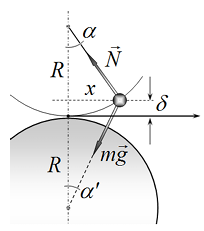
\includegraphics[width=0.6\textwidth]{Figures/P1/Fig 1.2S.png}
  \end{subfigure}
  \hfill
  \begin{subfigure}[b]{0.49\textwidth}
    \centering
    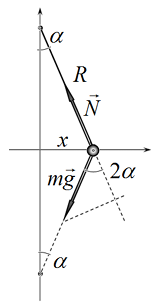
\includegraphics[width=0.4\textwidth]{Figures/P1/Fig 1.1S.png}
  \end{subfigure}
\end{figure}

\noindent\textbf{1.} Giả sử con lắc chuyển động trên quỹ đạo tròn, độ cao của con lắc so với mặt đất là
\begin{equation*}
  \delta=R-R\cos\alpha
\end{equation*}
với $\alpha$ là góc lệch của con lắc so với phương thẳng đứng. Với các góc lệch nhỏ, ta có:
\begin{equation*}
  \delta \approx \frac{\alpha^{2}}{2}R\approx 0
\end{equation*}
trong giới hạn này, ta có thể giả định:
\begin{itemize}
  \item con lắc di chuyển trên một đường thẳng;
  \item Các góc trên hình vẽ là bằng nhau;
  \item Trọng lực tác dụng lên con lắc không thay đổi và bằng $mg$, hướng về tâm Trái Đất.
\end{itemize}
Chiếu các lực lên phương sợi dây, ta có:
\begin{equation*}
  N=mg\cos 2\alpha\approx mg
\end{equation*}
và trên phương ngang:
\begin{equation*}
  ma_{x}=-2mg\sin\alpha\approx-2mg\alpha
\end{equation*}
ngoài ra:
\begin{equation*}
  x=R\alpha
\end{equation*}
suy ra:
\begin{equation*}
  x=\frac{g}{R}a_{x}
\end{equation*}
như vậy, chu kì chuyển động của con lắc là:
\begin{equation*}
  T=2\pi\sqrt{\frac{R}{g}}\approx 1 \text{ giờ}
\end{equation*}

